\documentclass{ximera}
\input{../preamble.tex}

\title{What Makes a Good Coordinate System?} \license{CC BY-NC-SA 4.0}

\begin{document}

\begin{abstract}
\end{abstract}
\maketitle

\begin{onlineOnly}
\section*{What Makes a Good Coordinate System?}
\end{onlineOnly}

\subsection*{How to Read a Coordinate System}
Let's take a fresh look at the familiar rectangular coordinate system.  We can impose such a coordinate system on a plane by picking the origin, and two orthogonal unit vectors $\vec{i}$ and $\vec{j}$ to determine the axes.  In the diagram on the left, the point $P=(3,2)$ can be located by moving 3 units from the origin in the direction of $\vec{i}$, then moving 2 units in the direction of $\vec{j}$. In this coordinate system, vector $\vec{v}$ drawn from the origin to point $P$, is represented by $\begin{bmatrix}3\\2\end{bmatrix}$.  We can express $\vec{v}$ as a linear combination of $\vec{i}$ and $\vec{j}$ as $\vec{v}=3\vec{i}+2\vec{j}$.  Note that the coefficients of the linear combination are the first and second components of $\begin{bmatrix}3\\2\end{bmatrix}$.

\begin{center}
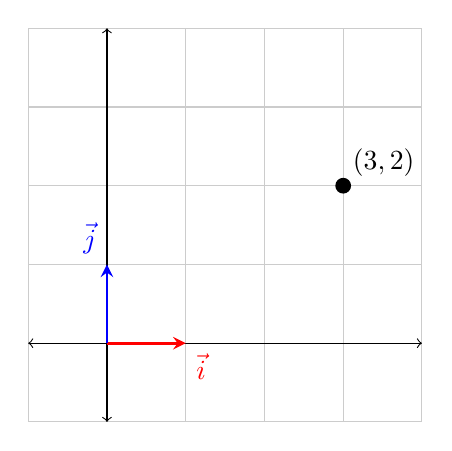
\begin{tikzpicture}[scale=1]
\draw[thin,gray!40] (-1,-1) grid (4,4);
  \draw[<->] (-1,0)--(4,0);
  \draw[<->] (0,-1)--(0,4);
  \fill[black] (3,2)node[above right]{$(3,2)$} circle (0.1cm);
   \draw[line width=1pt,-stealth, red](0,0)--(1,0) node[below right]{$\vec{i}$};
  \draw[line width=1pt,-stealth, blue](0,0)--(0,1) node[above left]{$\vec{j}$};
 \end{tikzpicture}\quad\quad\quad\quad
 \begin{tikzpicture}[scale=1]
\draw[thin,gray!40] (-1,-1) grid (4,4);
  \draw[<->] (-1,0)--(4,0);
  \draw[<->] (0,-1)--(0,4);
  \draw[line width=1pt,-stealth, red](0,0)--(1,0) node[below right]{$\vec{i}=\begin{bmatrix}1\\0\end{bmatrix}$};
  \draw[line width=1pt,-stealth, blue](0,0)--(0,1) node[above left]{$\vec{j}=\begin{bmatrix}0\\1\end{bmatrix}$};
  \draw[line width=1pt,-stealth, black](0,0)--(3,2) node[above]{$\vec{v}=\begin{bmatrix}3\\2\end{bmatrix}$};
 \end{tikzpicture}
\end{center}

Orthogonal unit vectors are often a convenient choice for establishing a coordinate system, but occasionally, using other vectors is preferable. An example of an alternative coordinate grid determined by vectors $\vec{v}_1$ and $\vec{v}_2$ is shown below.  

\begin{center}
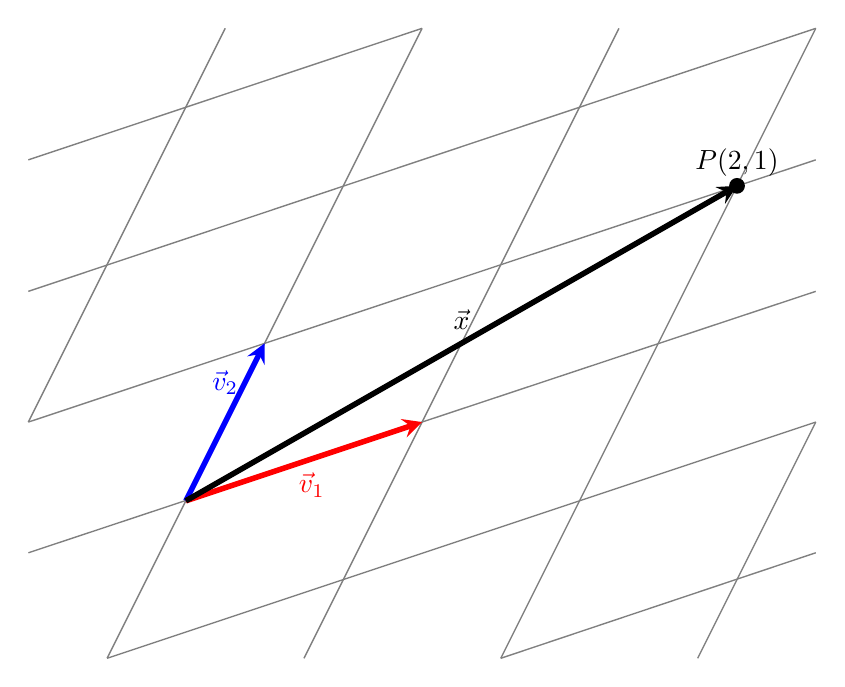
\begin{tikzpicture}[scale=1]
\draw[line width=0.5pt, gray](-2,1)--(0.5,6);  
\draw[line width=0.5pt, gray](-1,-2)--(3,6);
\draw[line width=0.5pt, gray](1.5,-2)--(5.5,6);
\draw[line width=0.5pt, gray](4,-2)--(8,6);
\draw[line width=0.5pt, gray](6.5,-2)--(8,1);
\draw[line width=0.5pt, gray](-2, 4.33)--(3,6);
\draw[line width=0.5pt, gray](-2, 2.66)--(8,6);
\draw[line width=0.5pt, gray](-2, 1)--(8,4.33);
\draw[line width=0.5pt, gray](-2, -0.66)--(8,2.66);
\draw[line width=0.5pt, gray](-1, -2)--(8,1);
\draw[line width=0.5pt, gray](4,-2)--(8,-0.66);
 \draw[line width=2pt,blue,-stealth](0,0)--(1,2);
\draw[line width=2pt,red,-stealth](0,0)--(3,1);
\draw[line width=2pt,-stealth](0,0)--(7,4);
\node[blue] at (0.5, 1.5)  (p2)    {$\vec{v}_2$};
\node[red] at (1.6, 0.2)  (p2)    {$\vec{v}_1$};
\node[] at (3.5, 2.3)  (p2)    {$\vec{x}$};
\fill[black] (7,4)node[above]{$P(2,1)$} circle (0.1cm);
 \end{tikzpicture}
 \end{center}

 Fortunately, finding points and constructing vectors in such coordinate systems relies on the same principles used in the familiar rectangular coordinate system. To reach point $P$, we start at the origin, then travel 2 copies of $\vec{v}_1$ in the direction of $\vec{v}_1$, followed by one copy of $\vec{v}_2$ in the direction of $\vec{v}_2$.  We can say that in this coordinate system, $P$ has coordinates $(2,1)$.  Also, observe that vector $\vec{x}$ can be written as a linear combination of $\vec{v}_1$ and $\vec{v}_2$ as follows $$\vec{x}=2\vec{v}_1+\vec{v}_2$$
 
 \begin{idea}
    We take it for granted that the $x$-coordinate (the coefficient in front of $\vec{i}$) is the first component in the ordered pair of coordinates, and the $y$-coordinate (the coefficient in front of $\vec{j}$) is the second component.  

    In the above setup, we chose to list the coefficient in front of $\vec{v}_1$ as the first coordinate of $P$ and the coefficient in front of $\vec{v}_2$ as the second coordinate.  

    How would the coordinates of $P$ be impacted if we had chosen a different order?  Think about why establishing (or knowing) the order in which $\vec{v}_1$ and $\vec{v}_2$ are used is important.
 \end{idea}

 \begin{exploration}\label{exp:readingCoords}

 The following interactive demonstrates how to find coordinates for a point using a coordinate grid defined using vectors $\overrightarrow{OA}$ and $\overrightarrow{OB}$ (in that order).
 
 To use the interactive
 \begin{itemize}
    \item Move the sliders to change the coordinates of $P$ within this coordinate system;
    \item Move the tips of vectors $\overrightarrow{OA}$ and $\overrightarrow{OB}$ to change the coordinate system.  
 \end{itemize}    
    
 \begin{question}
    Move the tips of vectors $\overrightarrow{OA}$ and $\overrightarrow{OB}$ to change the coordinate system.  Explain why the coordinates of $P$ do not change while $P$ moves around the plane.
 \end{question}    

% https://www.geogebra.org/classic/qxjtdgkc

\begin{center}
    \geogebra{qxjtdgkc}{800}{600}
\end{center}

\end{exploration}

\subsection*{Existence and Uniqueness of Representation}

We now understand that we can take two vectors and use them to impose a coordinate system on a plane.  In this section we will explore the properties of vectors that determine a ``good'' coordinate system.  The following questions will be central to our discussion:
\begin{itemize}
    \item Can ANY two vectors be used to form a coordinate system in a plane?
    \item Can we use more than two vectors to determine a coordinate system in a plane?
    \item What constitutes a ``good'' coordinate system?
\end{itemize}    


\begin{exploration}\label{exp:coordSystemLinCombs1}
Use the interactive below to answer the questions.  

Tip: To better navigate between the interactive and the questions, we suggest that you use a second device to manipulate the interactive.  Refresh your browser to reset the interactive to default settings.
% https://www.geogebra.org/classic/qw5dpmqq
\begin{center}
    \geogebra{qw5dpmqq}{800}{600}
\end{center}
\begin{question}
    Find the coordinates for each $P_i$ with respect to the given coordinate system.  Your coordinates should be of the form $(A\text{-coordinate}, B\text{-coordinate})$.
    $$P_1=\left(\answer{1},\answer{1}\right)$$
    $$P_2=\left(\answer{-2},\answer{0}\right)$$
    $$P_3=\left(\answer{0},\answer{-1}\right)$$
    $$P_4=\left(\answer{-2},\answer{3}\right)$$
    $$P_5=\left(\answer{3},\answer{-2}\right)$$
\end{question}

\begin{question}
Move point $B$ to coincide with $P_3$.
    List the coordinates for each $P_i$ with respect to the new coordinate system.  Your coordinates should be of the form $(A\text{-coordinate}, B\text{-coordinate})$.
    $$P_1=\left(\answer{1},\answer{-1}\right)$$
    $$P_2=\left(\answer{-2},\answer{0}\right)$$
    $$P_3=\left(\answer{0},\answer{1}\right)$$
    $$P_4=\left(\answer{-2},\answer{-3}\right)$$
    $$P_5=\left(\answer{3},\answer{2}\right)$$
    How do these coordinates compare to the coordinates in the previous question?  Explain why this is happening. (Hint: you can refresh your browser to return to the original coordinate system for comparison.)
\end{question}

\begin{question}
Refresh your browser to return to the original coordinate system.  Move point $A$ to coincide with $P_1$.
    List the coordinates for each $P_i$ with respect to the new coordinate system.  Your coordinates should be of the form $(A\text{-coordinate}, B\text{-coordinate})$.
    $$P_1=\left(\answer{1},\answer{0}\right)$$
    $$P_2=\left(\answer{-2},\answer{2}\right)$$
    $$P_3=\left(\answer{0},\answer{-1}\right)$$
    $$P_4=\left(\answer{-2},\answer{5}\right)$$
    $$P_5=\left(\answer{3},\answer{-5}\right)$$
    How do these coordinates compare to the coordinates in the original coordinate system?  Explain why this is happening. (Hint: you can refresh your browser to return to the original coordinate system for comparison.)
\end{question}

\begin{question}
    Refresh your browser to return to the original coordinate system.  Express each $\overrightarrow{OP}_i$ as a linear combination of $\overrightarrow{OA}$ and $\overrightarrow{OB}$.
$$\overrightarrow{OP}_1=\answer{1}\overrightarrow{OA}+\answer{1}\overrightarrow{OB}$$
$$\overrightarrow{OP}_2=\answer{-2}\overrightarrow{OA}+\answer{0}\overrightarrow{OB}$$
$$\overrightarrow{OP}_3=\answer{0}\overrightarrow{OA}+\answer{-1}\overrightarrow{OB}$$
$$\overrightarrow{OP}_4=\answer{-2}\overrightarrow{OA}+\answer{3}\overrightarrow{OB}$$
$$\overrightarrow{OP}_5=\answer{3}\overrightarrow{OA}+\answer{-2}\overrightarrow{OB}$$

Discuss the relationship between your answers to the first question and your answers here.  Observe that each vector $\overrightarrow{OP}_i$ is in $\text{span}\left(\overrightarrow{OA},\overrightarrow{OB}\right)$.
\end{question}

\begin{question}
    Move point $B$ to coincide with $P_2$.  What do you observe?  Can we express every point in the plane as a linear combination of $\overrightarrow{OA}$ and $\overrightarrow{OB}$? Do vectors $\overrightarrow{OA}$ and $\overrightarrow{OB}$ determine a good coordinate system for the plane? Can we express \textit{some} points in the plane as linear combinations of $\overrightarrow{OA}$ and $\overrightarrow{OB}$?  

    Write a short paragraph to recast your answers above in terms of \textit{span}.  Can we express every point in the plane as a linear combination of $\overrightarrow{OA}$ and $\overrightarrow{OB}$? Do vectors $\overrightarrow{OA}$ and $\overrightarrow{OB}$ span the plane?  Can we express \textit{some} points in the plane as linear combinations of $\overrightarrow{OA}$ and $\overrightarrow{OB}$?  What is the span of $\overrightarrow{OA}$ and $\overrightarrow{OB}$?
\end{question}

\end{exploration}

\begin{exploration}\label{exp:coordSystemLinCombs2}
We will use the same set-up as in the previous exploration but introduce an additional vector $\overrightarrow{OC}$.  Tips: To better navigate between the interactive and the questions, we suggest that you use a second device to manipulate the interactive.  Refresh your browser to reset the interactive to default settings.

 % https://www.geogebra.org/classic/b3k96x2w

 \begin{center}
     \geogebra{b3k96x2w}{800}{600}
 \end{center}

 \begin{question}
     Let's attempt to define a coordinate system using three vectors: $\overrightarrow{OA}$, $\overrightarrow{OB}$, and $\overrightarrow{OC}$.  If the coordinates are to be of the form $(A\text{-coordinate}, B\text{-coordinate}, C\text{-coordinate})$, how many ways do you think there would be to express $P_1$? Fill in the missing coordinates for $P_1$ below to get a sense of the variety of possibilities.
     $$P_1=\left(\answer{1},\answer{1},0\right)$$
     $$P_1=\left(0,\answer{2},\answer{0.5}\right)$$
     $$P_1=\left(\answer{2}, 0, \answer{-0.5}\right)$$
     $$P_1=\left(\answer{3},-1,-1\right)$$
 \end{question}

 \begin{question}
     Based on your work above, express $\overrightarrow{OP_1}$ as a linear combination of $\overrightarrow{OA}$, $\overrightarrow{OB}$, and $\overrightarrow{OC}$.  How many ways do you think there are to do this?
 \end{question}

 \begin{question}
     Compare and contrast the coordinate systems in this exploration and Exploration \ref{exp:coordSystemLinCombs1}.  
 \end{question}
    
\end{exploration}

We now return to the question of what makes a good coordinate system.  In this section we restricted our explorations to the plane but the same principles apply in other settings.  (What does a coordinate grid look like in $\RR^3$?)

\begin{idea}
    What makes a good coordinate system?
    \begin{itemize}
        \item Every point has coordinates associated with it;
        \item Each point has exactly one coordinate representation.
    \end{itemize}
\end{idea}

We can recast the above idea in terms of vectors.  First, the vectors that determine the axes must span the plane.  This would guarantee that every vector in the plane can be written as a linear combination of the axes vectors.  Second, we want that linear combination to be unique.  Exploration \ref{exp:coordSystemLinCombs1} demonstrates how picking two vectors that do not span the plane results in a bad coordinate system.  Exploration \ref{exp:coordSystemLinCombs2} shows that even when the axes vectors span the plane, using too many vectors as axes vectors results in loss of uniqueness of representation.
  
In the previous section, you learned how to address questions related to span. This will help you tackle existence of representation.  In the next section, we will address the question of uniqueness.
\end{document} 